{\color{indiagreen}\subsection{Newtnov gravitacijski zakon}}
(opisuje privlačno silo med dvema točkastema telesoma)\\
*smer sile je na smeri veznice
\begin{align*}
	F &= \frac{Gm_1m_2}{r^2}\\
\end{align*}
*če povečamo eno maso se obe sile povečata\\
G \dots gravitacijska konstanta\\
$G = 6,67 * 10^{-11} \frac{Nm^2}{kg^2}$\\
*vzamemo razdaljo med središčem\\

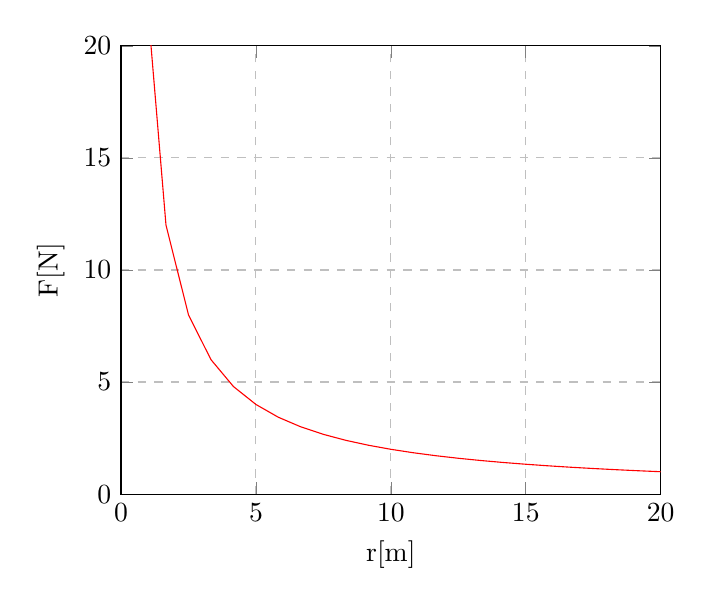
\begin{tikzpicture}
	\begin{axis}[
	    xlabel={r[m]},
	    ylabel={F[N]},
	    xmin=0, xmax=20,
	    ymin=0, ymax=20,
	    xtick={0,5,10,15,20},
	    ytick={0,5,10,15,20},
	    ymajorgrids=true,
	    xmajorgrids=true,
	    grid style=dashed,
	]
	 
	\addplot[domain=0:20,red] {20/x};

	\end{axis}
\end{tikzpicture}
\begin{enumerate}
	\item \textbf{MASA ZEMLJE}\\
		$g_0$ \dots težni pospešek na površini zemlje\\
		$r_0$ \dots polmer zemlje\\
		\begin{align*}
			mg_0 &= \frac{Gmm_z}{r_0^2}\\
			{\color{bostonuniversityred}g_0} &= {\color{bostonuniversityred}\frac{Gm_z}{r_0^2}}\\
			{\color{bostonuniversityred}m_z} &= {\color{bostonuniversityred}\frac{g_0r_0}{G}}\\
			m_z &= \frac{9,81\frac{m}{s^2}(6400km)^2}{6,67*10^{-11}\frac{Nm^2}{kg^2}} = 6,02*10^{24} kg\\
		\end{align*}
	\item \textbf{Težni pospešek nad površino zemlje}\\
		\begin{align*}
			{\color{bostonuniversityred}g} &= {\color{bostonuniversityred}g_0(\frac{r_0}{r}^2)} \dots od središča\\
			{\color{bostonuniversityred}g} &= {\color{bostonuniversityred}g_0(\frac{r_0}{r_0+h}^2)} \dots od površine zemlje\\
		\end{align*}
	\item \textbf{Hitrost umetnega satelita, ki kroži okrog zemlje na majhni višini}\\
		\begin{align*}
			{\cancelto{}{m}}g &= {\cancelto{}{m}}a_r\\
			g_0(\frac{r_0}{r})^2 &= \frac{v^2}{r}\\
			r &= r_0\\
			{\color{bostonuniversityred}v^2} &= {\color{bostonuniversityred}g_0r_0}\\
			v &= \sqrt{g_0r_0}\\
			v &= \sqrt{9,81\frac{m}{s^2}6400km}\\
			v &= 8000 \frac{m}{s} \rightarrow kozmična hitrost\\
		\end{align*}
		\textbf{Obhodni čas}:
		\begin{align*}
			v &= \omega r = \frac{2\pi}{t_0}r\\ 
			{\color{bostonuniversityred}t_0} &= {\color{bostonuniversityred}\frac{2\pi r}{v}}\\
			t_0 &= \frac{2\pi 6400km}{80000\frac{m}{s}} = 83,8 min
		\end{align*}
	\item \textbf{Višina geostacionarnega satelita}\\
		$t_0 = 1$dan $\rightarrow$ ker je goestacionarni satelit\\
		\begin{align*}
			\omega &= \frac{2\pi}{t_0}\\
			{\cancelto{}{m}}g &= {\cancelto{}{m}}a_r\\
			g_0(\frac{r_0}{r})^2 &= \omega^2 r\\
			g_0\frac{r_0^2}{r^2} &= \frac{4\pi^2}{t_0^2}r\\
			{\color{bostonuniversityred}r^3} &= {\color{bostonuniversityred}\frac{g_0r_0^2t_0^2}{4\pi^2}}\\
			r &= \sqrt{\frac{9,81\frac{m}{s^2}(6400km)^2(24h)^2}{4\pi^2}}\\
			r &= 42354km\\
			h &= r - r_0 = 36100km
		\end{align*}
	\item \textbf{Masa sonca}\\
		\begin{align*}
			r_{sz} &= 1,5 * 10^8km\\
			t_0 &= 365dni = 32 *10^6s\\
			\frac{Gm_s{\cancelto{}{m_z}}}{r_{sz}^2} &= {\cancelto{}{m_z}}\omega r_{sz}\\
			\frac{Gm_s}{r_{sz}^2} &= \frac{4\pi^2}{t_0^2}r_{sz}\\
			{\color{bostonuniversityred}m_s} &= {\color{bostonuniversityred}\frac{4\pi^2 r_{sz}^3}{t_0^2 G}}\\
			m_s &= 2 * 10^{30}kg\\ 
		\end{align*}
\end{enumerate}